\documentclass[10pt,twocolumn,letterpaper]{article}

\usepackage{graphicx} % Required for inserting images
\usepackage{kotex}
\usepackage{booktabs}
\usepackage[bookmarks,bookmarksnumbered]{hyperref}
\usepackage{hyperref}
\usepackage{graphicx}
\usepackage{amsmath}
\usepackage{amssymb}

 

\hypersetup{
    colorlinks=true,
    linkcolor=red,
    filecolor=magenta,      
    urlcolor=cyan,
}
 

\title{Object detection for defect detection}
\author{Kim Ji Won , Jung Hyunjin , Kim Young-soon}
\date{May 2023}
\begin{document}


\maketitle
\begin{center}
\begin{abstract}
  Transformer 구조는 현재 computer vision 분야에서 다양한 방식으로 사용되고 다양한 문제를 해결해오고 있다.
  attention이라는 개념을 필두로 CNN의 기본 가정을 무시하고 object detection에서 뛰어난 성능을 보이고 있다.
  이에 따라서 구리 축관 예측 문제에서도 Transformer를 사용해 성능 향상을 하려한다.
\end{abstract}
\end{center}

\section{Introduction}
4차 산업혁명은 제조업뿐만 아니라 다양한 산업 분야에서도 큰 변화를 가져오고 있다. 인공지능, 빅데이터, 클라우드 컴퓨팅, 로봇 공학 및 사물인터넷(IoT) 등의 기술을 기본으로 하며, 기존의 산업 구조를 완전히 변화시키고 새로운 경제 성장 모델을 창출한다. 4차 산업혁명으로 인해 스마트 팩토리 같은 첨단화된 제조공정은 대부분 자동화되어 제품을 대량 생산하고 있다. 
스마트 팩토리는 생산 공정을 자동화하여 생산성을 향상시키고, 스마트 팩토리의 세 가지 핵심 요소는 사물인터넷, 클라우드 컴퓨터, 빅데이터 분석기술이다.  삼성전자, Intel, Siemens 등 다양한 기업들이 생산 프로세스 개선과 생산성 증가를 위해 스마트 팩토리를 도입하고 있다. 생산 라인의 자동화, 생산 데이터의 수집과 분석, 로봇 기술 등을 활용하여 생산 공정을 최적화한다. 삼성 전자는 스마트 팩토리 도입으로 생산성이 15\% 향상되었고, Siemens의 경우 생산 라인의 운영 시간이 20\% 증가했다. 이러한 예는 생산 프로세스 개선을 목적으로 하는 기업들이 스마트 팩토리 도입을 통해 얻을 수 있는 잠재적 이점을 보여준다. 
컴퓨터 비전 기술을 이용한 산업용 시각 검사는 수십 년간 고려되어온 접근 방식이다. 최근 딥러닝의 발전으로 인해 단순한 환경에서부터 복잡한 환경에서까지 자동 시각 검사가 가능해졌다. 딥러닝 기반의 컴퓨터 비전에서 컨벌루션 신경망(CNN)은 최근 10년간 컴퓨터 비전 분야의 대표적 방법이었다. Abushahma 외(2019)는 객체탐지(Object Detection) 분야에서 R-CNN과 그 파생 모델들의 개념과 구조를 자세히 설명하고,Faster R-CNN, RPN 등을 활용하여 객체 탐지의 정확도와 속도를 향상시킨다 . 
뿐만 아니라 최근 등장한 어텐션 기반 비전 트랜스포머 아키텍처는 이미지 분류, 객체 탐지, 세분화와 같은 일반적인 컴퓨터 비전 작업에서 CNN을 능가하는 결과를 보여주었다. 그러나 뛰어난 성능에도 불구하고, 비전 트랜스포머를 실제 산업용 시각 검사에 적용하는 경우는 드물다. 이는 해당 방법들이 효과적으로 작동하기 위해서는 막대한 양의 데이터가 필요하다는 가정 때문인 것으로 보인다.
본 연구의 분석 목적은 실제 공정 이미지 자료를 통한 용접의 결함 여부를 분류하는 것이다. 제품의 표면 결함 이미지는 제품에서 용접을 기준으로 전공정과 후공정으로 나누어 20일 간의 총 31,193개 자료가 수집되었다. 그 중 1231개의 불량데이터가 있으며, 불량 데이터 Figure \ref{dataset}은 과적합과 미적합으로 분류된다. 
\begin{figure}[t]
  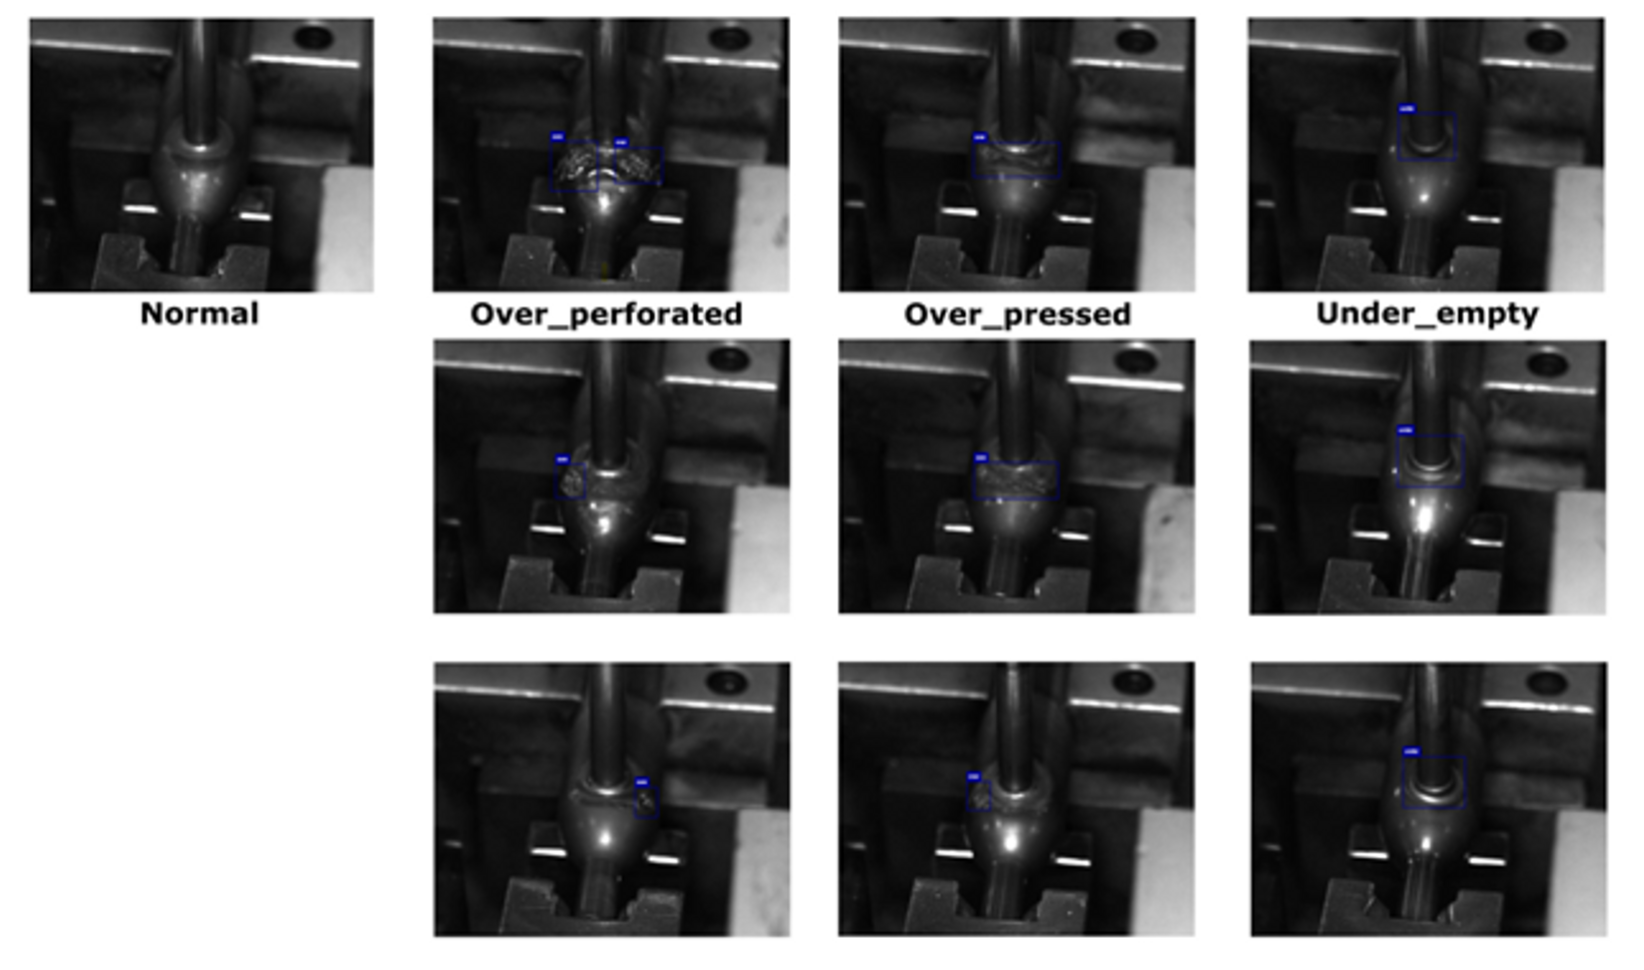
\includegraphics[width=\linewidth]{figure/dataset}
     \caption{\small \textbf{Class label} }
  \label{dataset}
  \end{figure}


\section{Related work}
\subsection{Defect detection}
결함감지는 4차 산업 혁명 시대에 가장 중요한 task 중 하나이다.
머신러닝 부터 딥러닝 까지 다양한 method를 활용해 정확도를 올려왔고
이에따라 우리도 사용하려고 한다.
\subsection{CNN approaches}
AlexNet이 소개된 이후로, CNN을 활용한 object detection은 점진적으로 defect detection에 
확장되기 시작했다. VGG와, Resnet을 활용한 detection은 성능이 좋았고, 
여기서는 VGG-16을 classification에 사용했다.
Ale 외(2018)는 RetinaNet 모델을 사용하여 도로상의 손상을 자동으로 탐지하는 방법을 제안하였다 . 데이터 증강 및 클래스 가중치 조절 등의 기술을 추가로 활용하여 기존 방법들보다 높은 정확도와 빠른 속도를 동시에 달성하였다. 위 모델은 의학 분야에서도 활용되었다. Tiwari 외(2022)는 YOLO와 RetinaNet을 앙상블하여 X-선 이미지에서 COVID-19 병변을 감지하는 방법을 제안하였다

\subsection{transformer approaches}
더 최근에는 Transformer 모형 구조가 점진적으로 computer vision task에 사용되고 있었다.
이러한 모형들은 최근에 ViT나 Swin transformer등에 적용되며 state-of-the-art를 만들었고 
우리의 task 역시 Object detection에 주안점을 둔다.

\section{Method}

\subsection{Data sampling}

우리의 데이터셋은 over와 under 두가지 class에 대해서 Detection을 진행한다.
1월1일 부터 1월 31일 까지 3,1000개의 구리축관에 대해 결함 감지를 진행한다.
하지만 imbalance 문제로 인해 우리는 복원 추출과 비복원 추출을 함께 mini-batch에다가 적용하며 
데이터셋 불균형 문제를 해결하려 한다. dataset에 따라서
\begin{figure}[h]
  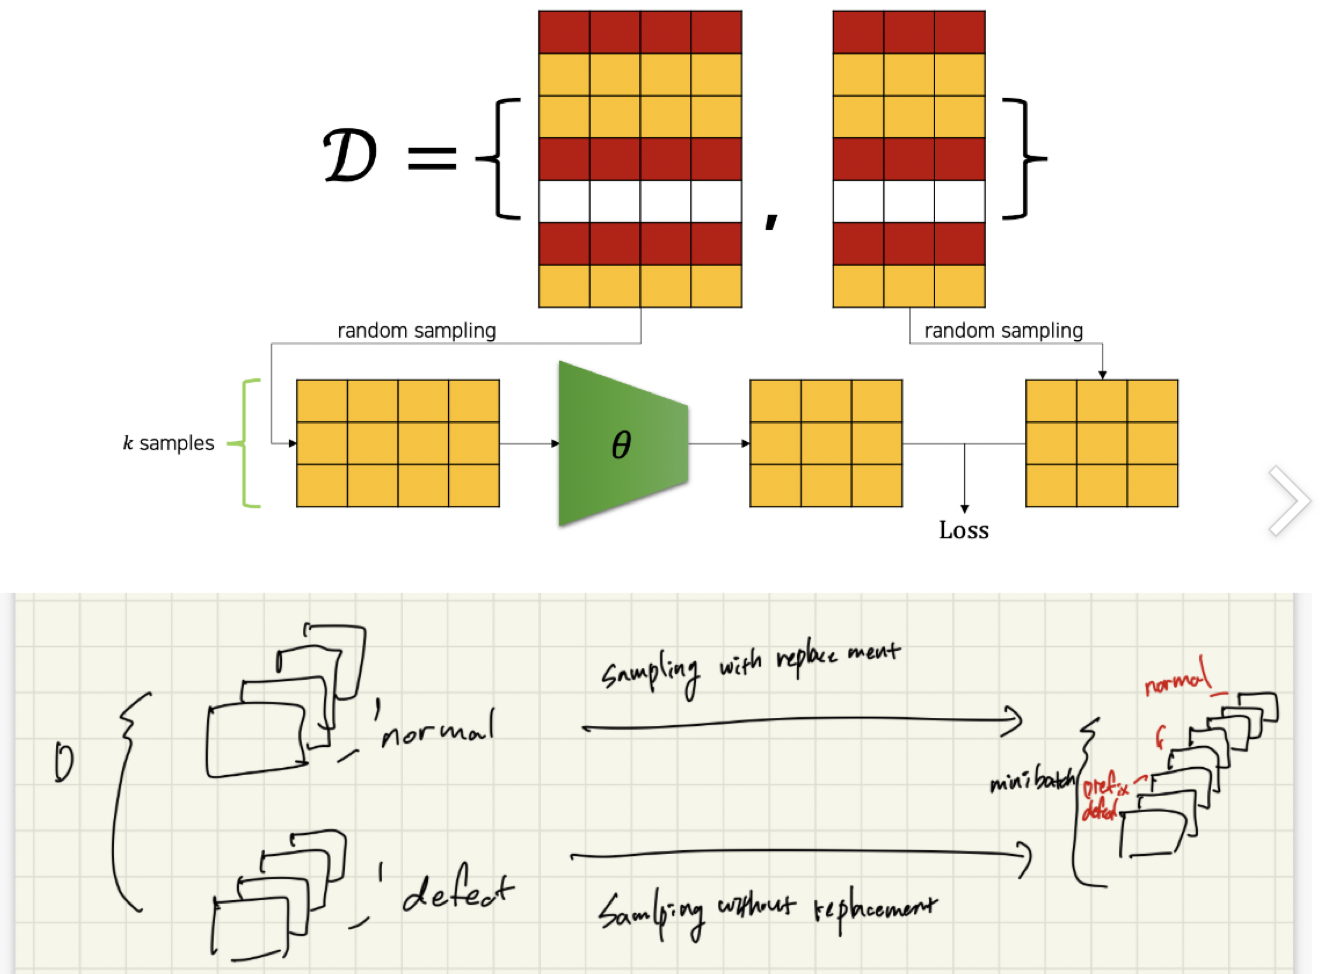
\includegraphics[width=\linewidth]{figure/data_sampling}
     \caption{\small \textbf{sampling} }
  \label{sampling}
  \end{figure}

\subsection{Anchor Generator}
\begin{figure}[htp!]
  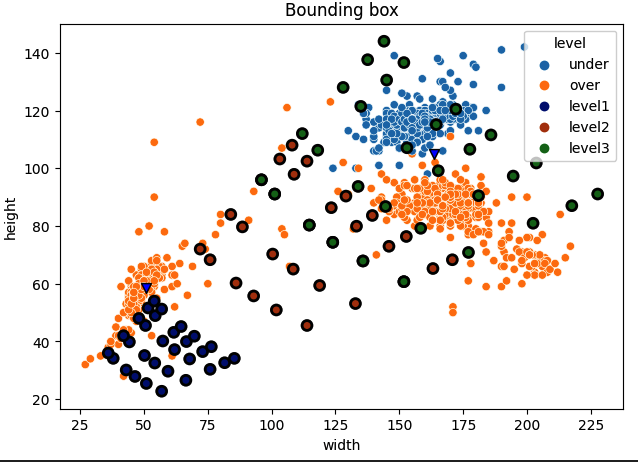
\includegraphics[width=\linewidth]{figure/anchor}
     \caption{\small \textbf{anchor} }
  \label{anchor}
  \end{figure}
정확도를 향상시키기 위해 사전 bounding box를 만들었다.
level 1 , level 2 , level 3를 나눠 anchor generator Figure \ref{anchor}를 통해 anchor를 생산하고 최대한 분포를 담을 수 있게 했다.
\subsection{Swin Transformer}
Swin transformer\cite{liu2021swin}를 활용해 우리는 모형을 적용했다.
swin transformer 모형은 CNN에 비해 예측력이 높고 inductive bias 문제만 해결한다면 다양한 문제를 해결할 수 있다.




\subsection{Losses}
\textbf{bounding box losses}\cite{r-cnn} 우리는 상대적인 좌표로 예측할 예정이기 때문에 아래와 같은 수식을 사용했다.
\begin{align}
  \begin{split}
    \hat{G}_x &=P_w d_x(P)+P_x \\
    \hat{G}_y &=P_h d_y(P)+P_y \\
    \hat{G}_w &=P_w \exp \left(d_w(P)\right) \\
    \hat{G}_h &=P_h \exp \left(d_h(P)\right)
  \end{split}
\end{align}
\begin{align}
  \begin{split}
  t_x  &=\left(G_x-P_x\right) / P_w \\
  t_y  &=\left(G_y-P_y\right) / P_h \\
  t_w  &=\log \left(G_w / P_w\right) \\
  t_h  &=\log \left(G_h / P_h\right)
  \end{split}
\end{align}

\textbf{bbox losses} where $t_{\star} = (t_{x},t_{y},t_{w},t_{h})$
\begin{equation}
L1\ loss=\sum_{\star=1}^n\left|t_{\star}\right|
\end{equation} 
\textbf{Class losses}\cite{retinanet}

\begin{align}
  \begin{split}
  p_t = 
  \begin{cases}
  p, & if \; \;  y=1 \\
  1-p
  & otherwise,
  \end{cases} \\ 
  FL(p_t)=-\alpha_t{(1-p_t)}^{\gamma}\log(p_t)
  \end{split}
  \end{align}
  

\textbf{Total Losses}
\begin{align}
  \begin{split}
   \lambda_{confidence}\sum_{i=0}^{S^2}\sum_{j=0}^{B} \mathbb-\alpha_t{(1-p_t)}^{\gamma}\log (p_t) \\ 
    + \lambda_{localization} \sum_{i=0}^{S^2}\sum_{j=0}^{B} 1_{ij}^{obj}|t_{\star}|
  \end{split}
\end{align}
\subsection{overall Architecture}
전체적인 architecture는 swin-L-fpn-retina\cite{fpn}이다.
feature pyramid network와 retina-net을 사용해서 만들었다.
\begin{figure*}[ht!]
  \centering
    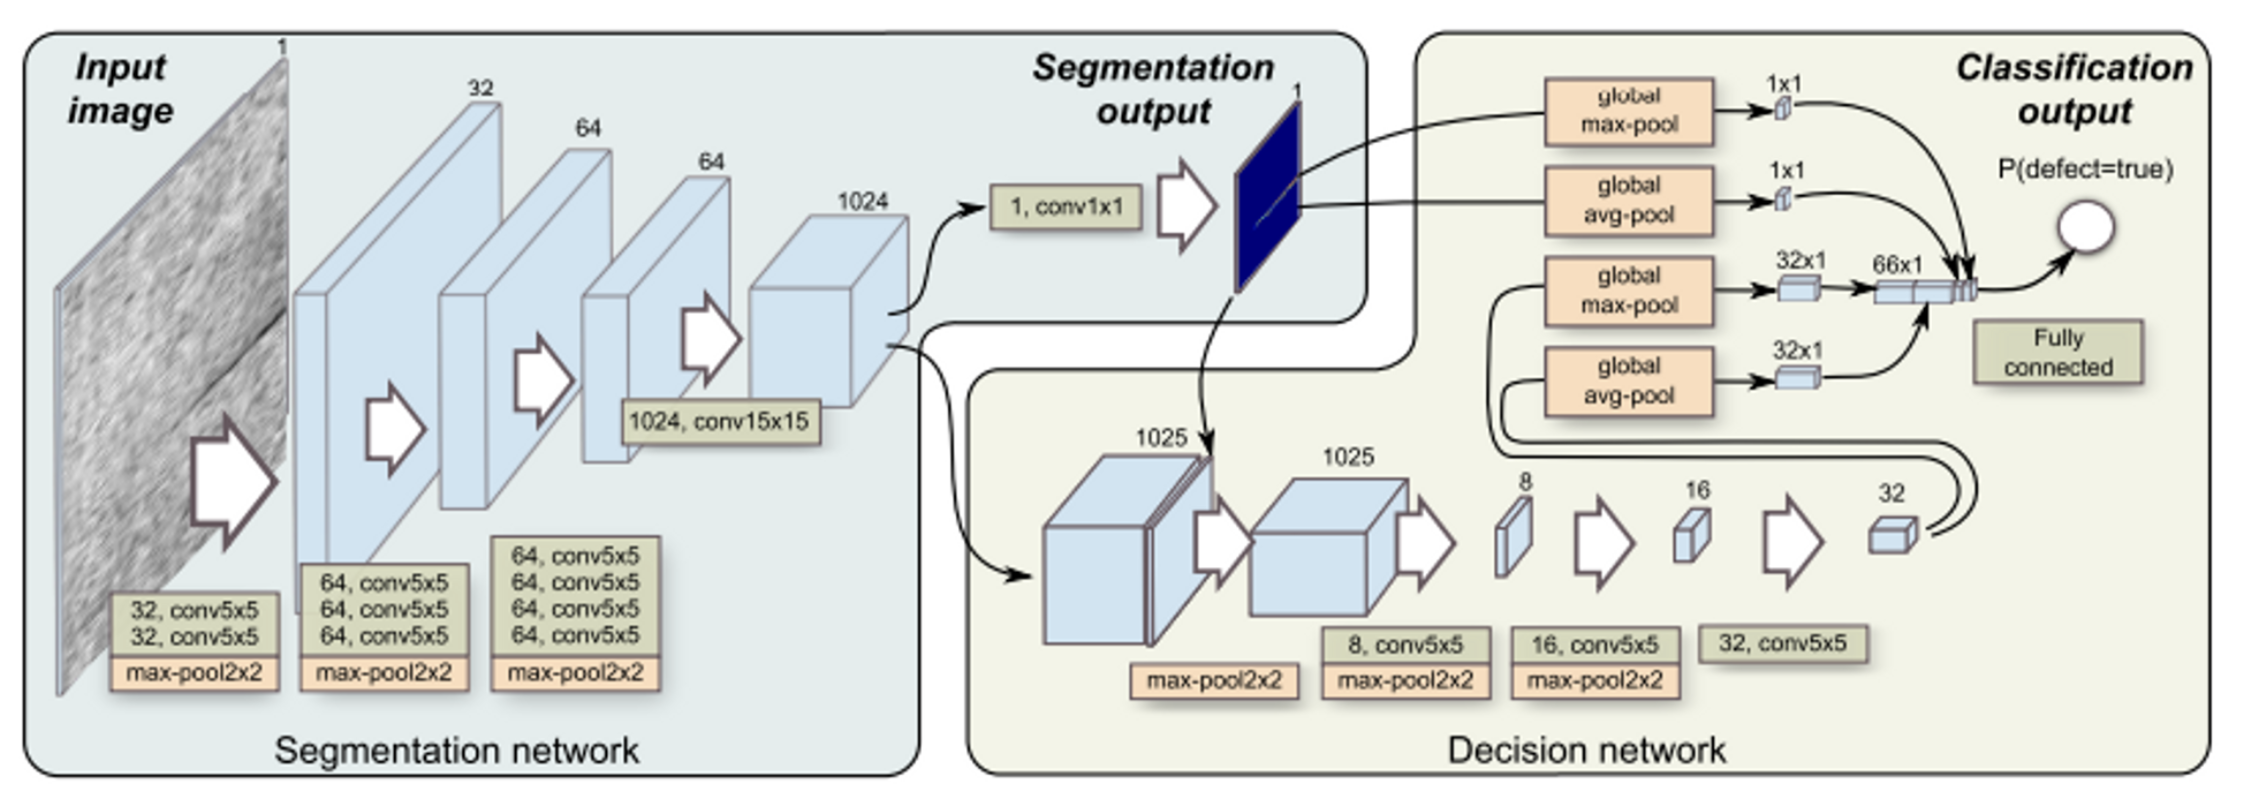
\includegraphics[width=.8\linewidth]{figure/model}
  \caption{\small \textbf{The Architecture.} overall architecture}
  \label{architecture}
\end{figure*}


\section{Experiments}
본 연구에서는 custom dataset으로 24,000장의 학습 데이터, 6,000의 검증 데이터 셋으로 구성되었고 결함이 있는 데이터는 1.2\%이다.
optimizer로 AdamW\cite{AdamW}를 사용하였고 초기값은 ${10}^{-5}$, weight decay ${10}^{-2}$를 기본값으로 사용하였다.
schedular는 cosine annealing을 사용했고 warm-up은 5,000 iterations 을 사용하였고 input size는 $512\times 512$로 통일 하였다.
backbone 모형은 ImageNet-1K를 활용하여 전이학습을 진행하였다.
Augumentation으로는 Horizontal Filip과 , [0,90] Range의 Rotation을 진행했다.
Epoch은 50번

\begin{table}[ht]  
\begin{center}
\begin{tabular}{|l|l|l|l|}
\toprule
mini batch size      & ${AP}_{50}$ & Precision & Recall \\ \midrule
defect sampling 5    & 93.39 & 80.30     & 95.60   \\
defect sampling 3    & 96.39 & 83.30     & 98.60   \\
defect sampling 2    & 92.30 & 81.30     & 93.60   \\  \bottomrule
\end{tabular}
\caption{Results of Object detection validation set by different sampling}\label{exp:minibatch}
\end{center}
\end{table}
\subsection{Defect sample size}
mini batch 중 어느 정도의 비중으로 mini batch를 구성하는지 좋을지에 대한 연구에서는 
Table~\ref{exp:minibatch}에서 보는 것과 같이 mini batch에서 3개를 넣었을 때 가장 좋은 결과가 나왔다.

\begin{table*}[tp]
  \centering
\begin{tabular}{|l|l|l|l|l|l|l|l|}
    \toprule
  Model                  & AP50 & AP\_over & AP\_under & Precision & Recall & params & FLOPS \\ \midrule
  ResNet152-FPN-Retina   & 92.59   & 92.59  & 92.59 & 83.03   & 89.23 & 17.5M & 20G    \\ 
  ResNet152-PAFPN-Retina & 92.06   & 92.06  & 92.06 & 86.68   & 86.84  & 17.5M & 20G   \\ 
  SwinL-FPN-Retina       & \textbf{96.39}   & 96.39  & 96.39 & 83.30   & 98.60 & 17.5M & 20G      \\ 
  SwinL-PAFPN-Retina     & 94.46   & 94.46  & 94.46 & 93.35   & 94.52  & 17.5M  & 20G  \\  
  EffNet-FPN-Retina       & \textbf{96.39}   & 96.39  & 96.39 & 83.30   & 98.60 & 17.5M & 20G      \\ 
  EffNet-FPN-Retina       & \textbf{96.39}   & 96.39  & 96.39 & 83.30   & 98.60 & 17.5M & 20G     \\ \bottomrule
  ResNet152-FPN-Dense   & 92.59   & 92.59  & 92.59 & 83.03   & 89.23 & 17.5M & 20G    \\ 
  ResNet152-PAFPN-Dense & 92.06   & 92.06  & 92.06 & 86.68   & 86.84  & 17.5M & 20G   \\ 
  SwinL-FPN-Dense       & \textbf{96.39}   & 96.39  & 96.39 & 83.30   & 98.60 & 17.5M & 20G      \\ 
  SwinL-PAFPN-Dense     & 94.46   & 94.46  & 94.46 & 93.35   & 94.52  & 17.5M  & 20G  \\  
  EffNet-FPN-Dense       & \textbf{96.39}   & 96.39  & 96.39 & 83.30   & 98.60 & 17.5M & 20G      \\ 
  EffNet-FPN-Dense       & \textbf{96.39}   & 96.39  & 96.39 & 83.30   & 98.60 & 17.5M & 20G     \\ \bottomrule
  \end{tabular}
  \caption{Results of Object detection validation set by different sampling}\label{exp:model}
  \end{table*}
\subsection{Results}
Table~\ref{exp:model} transformer based 모형을 사용하는 것이 가장 좋은 결과가 나왔다.
우리는 defect detection task 관련해서 swin transformer가 효과적인지 확인하기 위해 Resenet 관련 모형과 비교하였다.
그 결과 5가지 평가지표에 대해 모두 좋았다.
\section{Conclusion}
우리는 이러한 결과를 활용하여 구리 축관 결함 탐지에서도 swin transformer가 잘 작동한다는 것을 알 수 있었다.
본 감지는 3개의 레일에서 11초당 하나의 구리축관을 생산하기 때문에 목표 FPS는 0.3이었다.
따라서 초당 FPS가 1초가 채 되지 않는 Swintransformer 모형의 적용은 충분하다.


{\nocite{*}
\bibliographystyle{unsrt}
\bibliography{main.bib}
}
\end{document}